%\documentclass{sig-alternate}
%\documentclass{sig-alt-hotnetscr}
%\documentclass{sig-alternate-10pt}
\documentclass{sig-alternate-tight-10pt}

\usepackage{url,graphicx,multirow,hyperref,color,calc,ulem,threeparttable,tabularx,booktabs,enumitem,comment,balance}
\usepackage[group-separator={,}]{siunitx}

\hypersetup{%
  bookmarks=true,
  unicode=true,
  pdftoolbar=true,
  pdfmenubar=true,
  pdffitwindow=true,
  pdfstartview={FitV},
  pdftitle={},
  pdfauthor={},
  pdfnewwindow=true,
  colorlinks=false,
  pdfdisplaydoctitle=true,
  pdfborder={0 0 0},
}

\usepackage[all]{hypcap}

\usepackage[absolute]{textpos}

\setlist[itemize]{leftmargin=*}

\setlength{\TPHorizModule}{1in}
\setlength{\TPVertModule}{1in}
\textblockorigin{0.75in}{0.5in}

\newcommand*{\refname}{References}

\newcommand{\subparagraph}{}
\usepackage{titlesec}
%\titlespacing*{\section}{0pt}{3mm}{1mm}
\titlespacing*{\subsection}{0pt}{2mm}{1mm}
\titlespacing*{\subsubsection}{0pt}{1mm}{1mm}

\usepackage{subcaption}

\input{.xxxnote}
\input{.draft}
\input{.blue}
% 16 Nov 2010 : GWA : Any special macros or other stuff for this particular
%               paper go here.

\newcommand{\PhoneLab}{\textsc{PhoneLab}}
\hyphenation{Phone-Lab}



\begin{document}

\conferenceinfo{HotNets'14,}{October 27--28, 2014, Los Angeles, CA, USA.}
\CopyrightYear{2014}
\crdata{978-1-4503-3256-9}
\clubpenalty=10000
\widowpenalty = 10000

\def\thetitle{Crowdsourcing Access Network Spectrum Allocation Using Smartphones}
\title{\thetitle}

\author{%
  Jinghao Shi$^\dag$, Zhangyu Guan$^\dag$$^\S$, Chunming Qiao$^\dag$, Tommaso
  Melodia$^\S$\\ Dimitrios Koutsonikolas$^\dag$ and Geoffrey
  Challen$^\dag$\\[0.1in]
  {\large$^\dag$Department of Computer Science and Engineering, University at Buffalo}\\
  {\large $^\S$Department of Electrical and Computer Engineering, Northeastern University}\\[0.1in]
  $^\dag$\email{\large \texttt{\{jinghaos,zguan2,qiao,dimitrio,challen\}@buffalo.edu}},
  $^\S$\email{\large \texttt{melodia@ece.neu.edu}}
}

\hypersetup{
  pdfinfo={
    Title={\thetitle},
    Author={Jinghao Shi, Zhangyu Guan, Chunming Qiao, Tommaso Melodia, Dimitrios Koutsonikolas and Geoffrey Challen}
  },
}

\maketitle

\begin{abstract}

\sloppypar{The hundreds of millions of deployed smartphones provide an
unprecedented opportunity to collect data to monitor, debug, and continuously
adapt wireless networks to improve performance. In contrast with previous
mobile devices, such as laptops, smartphones are \textit{always on} but
\textit{mostly idle}, making them available to perform measurements that help
other nearby active devices make better use of available network resources.
We present the design of \textsc{PocketSniffer}, a system delivering wireless
measurements from smartphones both to network administrators for monitoring
and debugging purposes and to algorithms performing real-time network
adaptation. By collecting data from smartphones, \textsc{PocketSniffer}
supports novel adaptation algorithms designed around common deployment
scenarios involving both cooperative and self-interested clients and
networks. We present preliminary results from a prototype and discuss
challenges to realizing this vision.}

\end{abstract}

\category{C2.3}{Network Operations}{Network management}
\terms{Management, Performance}
\keywords{Smartphones, crowdsourcing, monitoring}

\section{Introduction}

Smartphone technologies are advancing rapidly, bringing power into users
pockets that is changing the way we live. The rapid rate at which consumers
purchase new smartphones can be seen as primarily a response to the speed at
which this technology is improving. Short device lifetimes, while unfortunate
from a sustainability perspective, help support companies that build and sell
smartphone hardware and software. Unfortunately smartphones, like most other
electronics, are difficult to dispose of properly. Many end up unused in desk
drawers, discarded in landfills, or shipped to poor countries where they are
dangerously dismantled in an effort to extract precious metals.

Given smartphones' current role in bringing about transformative
technological change, it is hard to argue that consumers should hang on to
outdated devices in the name of sustainability. Instead, we believe it will
be more effective to focus on how to reuse the devices we currently discard.
There are three reasons why the time is right for this effort. First, unlike
previous generations of ``feature phones'', the smartphone market is
coalescing around a small set of platforms, with this homogeneity reducing
the burden of reusing discarded devices. Today, each phone in an electronics
recycling bin runs a different OS; in three years, half of the smartphones in
the same bin may run Android.

Second, current smartphones have an attractive feature set for many non-phone
applications: size and power requirements facilitating easy deployment;
microphones, cameras, and other sensors built-in; touch screens for
interacting with users. And the volume at which they are produced combined
with the rate at which consumers are replacing them produces an extremely
competitive price point for discarded devices given their capabilities.

Finally, smartphones are well-integrated into existing communication
infrastructures. They can transmit data using text messages, Wifi networks,
and high-speed mobile communication technologies like 3G. If Wifi is
available, no service plans are required to allow recycled smartphones to
become part of the ``Internet of Things''. And with carriers increasingly
interested in ``machine-to-machine'' applications~\cite{sprint-m2m}, we
expect to see increasing service flexibility allowing discarded devices to be
cheaply connected to pervasive mobile cellular and data networks.

To provide an idea of the potential of discarded devices, the U.S.
Environmental Protection Agency (EPA) estimates that 141~million mobile
devices became ready for end-of-life management in 2009, of which only 11.7
million (8\%) were collected for recycling~\cite{epa-ewasteweb}. The
129~million discarded phones are enough to place an average of \textit{200
phones} on all 600,000~bridges in the United States, or one phone every
\textit{2~feet} on every mile of the 46,876~mile US interstate system.

In this paper, we investigate reusing smartphones sensor network ``motes''.
Compared to motes, discarded smartphones have many advantages, which we
outline in Section~\ref{sec-comparison}. And while power consumption is a
concern and the discarded phone's major weakness, we show in
Section~\ref{sec-results} that a simple and unoptimized sense-and-send
application running on a Nexus~S phone can last over a week on a full battery
charge, even while preserving the familiar and powerful Android programming
environment. To begin, the next section reviews the current state of
smartphone sustainability.

\newpage
\section{PocketSniffer Design}
\label{sec-design}

This section describes the design of \PS{}, a system enabling CANSAS for Wifi
networks by providing the client-side measurements needed to enable the
coordination algorithms described in the next section. We begin with an
overview of the \PS{} system from the perspective of a network user.

\subsection{Overview}

When Alice and Bob register for their campus WLAN they are required to
install the \PS{} monitoring app on their smartphones. As they travel around
campus, their smartphones collect measurements on the health and performance
of the campus network based on queries established by network administrators,
reporting these measurements in an energy-neutral way by uploading data only
when their smartphones are charging. Network administrators can use this data
to identify poorly-served areas of campus, locate APs that are over- or
underutilized, and for other network monitoring and debugging purposes.

In addition, as Alice and Bob sit together in a campus cafe using the campus
WLAN to surf the web---Alice on her tablet, Bob on his smartphone---suddenly
a new source of interference begins to disrupt their network performance.
Unfortunately this interfering terminal cannot be overheard at the AP they
are associated with, but the AP can tell that Alice's and Bob's networking
environment has degraded. At this point, it triggers the \PS{} app on Alice's
inactive smartphone to search for a less-congested channel. Based on the
results \PS{} may move their active devices to a different channel, adjust
the AP power level, or suggest they associate with a different campus AP, all
without performing measurements on their active clients that could interrupt
their web browsing. Without collecting measurements directly from Bob's
smartphone, \PS{} is still able to exploit the proximity between Alice and
Bob and use Alice's nearby inactive smartphone to estimate the impact of
changes on Bob's active smartphone to ensure that any spectrum adaptation
benefits both devices.

Later, when Alice and Bob return home to neighboring apartments their
overlapping home Wifi networks use \PS{} measurements as inputs to perform
cooperative spectrum allocation. Despite the lack of centralized control,
their two networks jointly adapt to allocate spectrum in a way that improves
performance for both Alice and Bob.

\subsection{Performing Measurements}
\label{subsec-measurement}

\PS{} collects two types of measurements from terminals---scan results and
spectrum utilization information---in two different ways---asynchronously and
synchronously.

\subsubsection{Measurement types}

Scan results are inexpensive to collect and provide a high-level view of the
network including visible APs and their signal strengths. Android smartphones
already perform Wifi scans at regular intervals, even while associated with a
Wifi network. Recovering this data incurs no energy overhead for clients as
long as the measurements are only uploaded while the battery is charging, and
our recent analysis of 89~million scan results collected from 139~smartphones
over 5~months~\cite{conext14-pocketsniffer} has demonstrated the value of
these measurements for network monitoring and debugging.

However, because smartphones are frequently idle, periodic scans may not
reflect either locations where users actually use their devices or locations
where their devices use the network. To better connect Wifi scans with
interactive usage and network activity, \PS{} annotates each scan with two
pieces of information: (1) whether the scan was performed during interactive
use as estimated by the screen state, and (2) the timestamp since device's last
data transfer, because not every interactive session includes Wifi usage and
because smartphones perform background data transfers with the screen
disabled.

In contrast, spectrum utilization measurements are expensive to collect and
may not be possible to collect on all clients, but provide a very detailed
view of spectrum usage. The ability of Wifi chipsets to observe link-layer
signaling traffic and packets sent by other terminals varies from device to
device, and because these measurements require disabling the power-save mode
used by mobile Wifi chipsets they consume extra energy even if measurement
upload is performed in an energy-neutral way. We discuss several research
challenges caused by Wifi chipset heterogeneity in
Section~\ref{sec-challenges}.

\subsubsection{Query types}

Asynchronous measurements are used to perform network monitoring and as a
replacement for expensive site surveys in order to do spatial and temporal
spectral capacity planning. For asynchronous queries \PS{} allows clients to
publish measurements to subscriptions set up by network administrators, each
of which contains one or more queries describing requested measurements.

\PS{}'s queries allow administrators to configure both asynchronous and
synchronous data collection by restricting the type of data collected, the
devices that participate, APs or active devices to observe, and times during
which to perform measurements. Pushing queries to clients allows \PS{} to
limit the energy overhead of the measurement process, even for asynchronous
queries when the data can most likely be collected during charging sessions.
\PS{} avoids disturbing active sessions by waiting to perform asynchronous
data collection until a certain amount of time has elapsed since the last
interactive session.

To support both network monitoring and debugging over long timescales as well
as rapid network adaptation \PS{} uses both synchronous and asynchronous
queries. Asynchronous queries are configured by network administrators,
long-running, and satisfied through delay-tolerant upload. Synchronous
queries are initiated on-demand by APs, short-lived, and satisfied
immediately by participating clients. When an asynchronous query arrives
\PS{} clients can decide whether they should collect and return the requested
measurements, a decision that is determined by several factors:

\begin{itemize}

\item \textbf{Usage status.} Because the goal of \PS{} is to avoid disturbing
active sessions active clients will ignore synchronous queries.

\item \textbf{Relationships between terminals.} \PS{} allows users to
configure their app to always return data about other devices that they own.
Relationships between terminals can be manually configured through the app,
or a list of other devices associated with a given user can be retrieved from
the \PS{} service to assist this process.

\item \textbf{Proximity to active terminals.} \PS{} clients must determine
whether they can provide measurements approximating the network conditions
experience by the active clients included in the query. We return to the
challenge of proximity detection and the question of whether to perform
proximity detection in signal or physical space in
Section~\ref{sec-challenges}.

\item \textbf{Battery level.} Because \PS{} runs on energy-constrained
  devices clients are free to not participate if they are low on energy. The
  \PS{} app allows users to configure separate battery thresholds for queries
  related and unrelated to their other devices.

\end{itemize}

If the terminal decides to participate in the synchronous query, it performs
the measurements and sends them directly to the AP. Note that if measurements
made to satisfy synchronous queries also match existing asynchronous queries,
they will also be uploaded to the PocketSniffer subscription by the AP.

\section{Coordination Scenarios}
\label{sec-algorithms}

When performing network adaptation \PS{} is designed to support multiple
different coordination patterns between clients sharing the same WLAN and
between overlapping WLANs. In all cases \PS{} algorithms utilize crowdsourced
measurements from inactive smartphones to attempt to improve performance for
active client by controlling AP channel assignments, client associations, and
AP power levels and transmission rates. Depending on the scenario, clients
may behave selfishly or provide incorrect data in hopes of either avoiding
the energy overhead of performing measurements or improving their own network
performance at the expense of others.

We are using \PS{} to explore several different CANSAS coordination
algorithms including maximization and game-theoretic approaches designed to
enable cooperation in each of the following common scenarios. Because we are
still determining which algorithms work best at achieving the objectives
appropriate to each scenario, we focus the discussion below on describing the
objective and the associated challenges.

\subsection{Single Network, Cooperative Clients}

In the first case a single network serves a set of clients which are
cooperative in the sense that they are willing to work together to achieve a
single common objective. Thus, \PS{} can assume that clients are willing to
provide truthful measurements. Typical home Wifi networks serving multiple
mobile devices fall into this category. Because clients are cooperative and a
global objective is shared, this scenario lends itself to the simplest
coordination algorithms. One example uses \PS{} measurements to select a set
of network parameters maximizing the aggregate throughput of all clients; a
variant prioritizes interactive sessions by only maximizing throughput to
interactive clients.

\subsection{Single Network, Selfish Clients}

In the second case a single network serves a set of clients each of which
wishes to maximize its own performance. Typical enterprise Wifi networks fall
into this category. This scenario presents two new complications compared
with the previous one. First, we must formulate a notion of social utility
balancing both performance and fairness. Second, \PS{} cannot assume that
clients are willing to provide truthful measurements. They may intentionally
mislead the system to try to improve their own performance at the expense of
other clients, or attempt to avoid the energy overhead of performing
measurements. We are addressing these challenges in two ways, both by
designing mechanisms that incentivize clients to perform accurate
measurements and by utilizing \PS{}'s control of the network APs to validate
client measurements.

\subsection{Multiple Networks, Cooperative Clients}

In the third case multiple independently-administered networks serve
clients that will cooperate within each network. Thus, \PS{} can assume that
clients provide truthful measurements but that each network acts in a
self-interested fashion. Overlapping home Wifi networks each serving multiple
mobile devices fall into this category. We are attempting to address this
scenario by formalizing the problem as a noncooperative game between the
competing networks where each attempts to selfishly maximize one of the local
objectives described in the first scenario.

\subsection{Multiple Networks, Selfish Clients}

In the final case multiple independently-administered networks serve sets of
self-interested clients. Thus, \PS{} can neither assume that clients will
provide truthful measurements nor that the networks will not act selfishly.
Overlapping enterprise Wifi networks fall into this category. Because \PS{}
must arrange cooperation both between clients within each network and between
the overlapping networks, this represents the most challenging scenario. We
are attempting to address it by framing it as a two-level noncooperative game
where coordination occurs first between the networks and then between
clients.

\section{Preliminary Results}
\label{sec-results}

As mentioned previously, we have performed a detailed analysis of 89~million
scan results collected from 139~smartphones over 5~months in order to
validate the usefulness of these measurements already being collected by
smartphones\footnote{This work is under concurrent
submission~\cite{conext14-pocketsniffer}.}. Encouraged by these results, we
have built a prototype \PS{} system including both an Android smartphone app
and adaptive AP. Because we have already explored asynchronous analyses that
can be performed using scan results, our preliminary results below focus on
what additional offline analyses can be done with more detailed channel
utilization information (\S\ref{subsec-rogue}) and on a basic form of online
channel adaptation (\S\ref{subsec-channel}).

To collect detailed channel utilization information, Wifi cards need to be
put in monitor mode so that every decoded packet is delivered to upper
layer---not just ones addressed to the client itself. Unfortunately, few
smartphone Wifi chipsets currently support this feature out of the
box\footnote{In some cases monitor mode support can be achieved by modifying
the firmware or device driver~\cite{bcmon}.}, a challenge we return to in
Section~\ref{sec-challenges}. As a work around allowing us to explore the
potential inclusion of this feature on next-generation smartphone devices, we
equipped several Galaxy Nexus~\cite{galaxynexus} smartphones with external
Wifi dongles that include chipsets that can be put into monitor mode.
Table~\ref{tab:dongle} describes the Wifi dongle used in our experiments.

\begin{table}[t!]
  \centering
  \begin{tabular}{ll}
    \toprule
    \textbf{Model} & ALFA Network AWUS036H \\
    \textbf{Chipset} & RTL8187L \\
    \textbf{Connector} & $1\times2.4$GHz SMA \\
    \textbf{Antenna} & 2.5dBi rubber duck \\
    \textbf{Wifi Support} & 802.11b/g \\
    \bottomrule
  \end{tabular}
  \caption{Wifi dongle specification.}
  \label{tab:dongle}
  \vspace*{-0.1in}
\end{table}


\subsection{Rogue Access Points}
\label{subsec-rogue}

Rogue APs (RAPs) are unauthorized APs deployed in areas designed to be
covered by existing enterprise wireless networks. RAPs are of concern to
network administrators both for security reasons and due to the unwanted
interference they may cause by competing with the official network for
spectrum resources. However, RAPs may be set up by users that feel
poorly-served by the official wireless network and if properly configured
they may not cause harmful interference. And realistically, our typical
campus network consisting of several thousand APs also contains hundreds of
RAPs, many more than available IT staff can deal with. A system like
\PS{} provides the ability to determine the impact of RAPs on clients'
network performance, allowing administrators to prioritize those that are
actually causing problems and ignore those that may be filling coverage
holes. To investigate the impact of RAPs, network administrators would
establish a \PS{} query asking devices to record short ($\sim$1~s) full packet
traces after scan results indicated the presence of a previously-identified
RAP.

Our department contains several RAPs. To investigate their impact, we
deployed 6~\PS{} devices: three were deployed statically in public areas,
with the remaining three carried by investigators for several hours each day.
All devices were put in continuous monitor mode in order to capture all
packet traffic, thus providing a superset of the data that would be provided
by actual \PS{} clients. In total, 38 device-hours worth of data containing
37~M packets were recovered. We first inspect beacon frames to identify APs.
Then we exclude campus APs and temporary hotspots with less than 1000~beacon
frames. 56~RAPs were detected in this way. For each RAP, we calculate the
total traffic volume (both down and up link) by summing up the length of all
data frames. Figure~\ref{fig:rap} shows 15 RAPs with most traffic, as well as
the number of devices that ever exchange data frames with them.


\begin{figure}[t!]
  \centering
  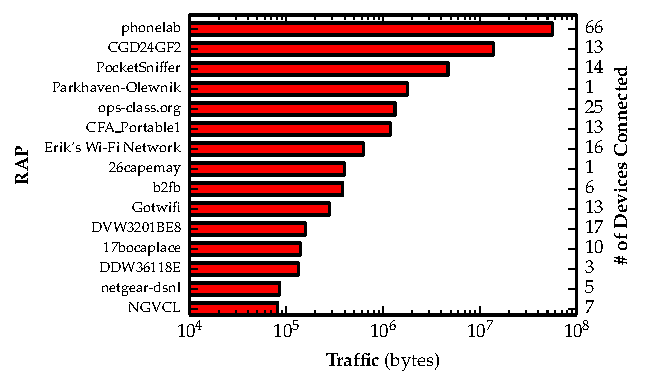
\includegraphics[width=0.48\textwidth]{./figures/RAPTrafficGraph.pdf}
  \vspace*{-0.15in}
  \caption{Measured Bandwidth to Rogue APs.}
  \label{fig:rap}
  \vspace*{-0.1in}
\end{figure}

Among these 15~RAPs \texttt{AP1}~and~\texttt{AP2}\footnote{These two AP SSIDs
have been changed for blind review.} are both operated by one of the
coauthors. \texttt{AP1} is unsecured which likely accounts for its higher
traffic volume and larger number of users, as it is available to users that
may not be able to authenticate to the campus network. \texttt{AP2} is
secured and only used by students in a particular room, and the large amount
of traffic it is serving might indicate a place where the campus network's
coverage could be improved. Other RAPs, such as \texttt{Parkhaven-Olewnik}
and \texttt{26capemay}, also generated large traffic volume yet all of them
are with one device, indicating personal RAPs that are secured and only used
by the owner.

\subsection{Channel Assignment}
\label{subsec-channel}

To demonstrate how \PS{} can enable realtime network adaptation to improve
the performance of nearby active clients, we ran an experiment using a
sniffer device and an adaptive AP. The AP periodically requests channel
measurements from all available channels from the sniffer and uses the data
to determine the least-congested channel.

The experiment is designed as follows. We first set up a constant
\texttt{iperf} UDP session between \PS{}-AP $AP$ and device $D_1$ on channel
$C_1$. Then another device $D_2$ starts jamming the channel using UDP traffic
to simulate a new and serious source of interference. However, because the AP
is periodically retrieving channel utilization statistics from the sniffer
device it can react to the interference by determining which other available
channel is the least congested. All of this happens without disturbing $D_1$
which continues transferring data. All devices in this experiment are using
802.11g at 2.4GHz band. In the particular run shown in Figure~\ref{fig:bw},
from 0--8.5~s $A$ and $D_1$ establish stable UDP traffic on channel 11.

When $D_2$ starts jamming the channel at 8.5~s the link bandwidth between $A$
and $D_1$ decreases and begins to fluctuate. At 75~s, when $A$ and $D_1$
switch to a less congested channel (1), the bandwidth resumes to the level
obtained before the interference began. The latency between the onset of the
interference and the channel switch is due to several factors, including the
time required for the AP to initiate measurements, the time required for the
device to perform the measurements, and the time required to transmit measurements to
the AP, all of which can be easily reduced in future prototypes.

\begin{figure}[t!]
  \centering
  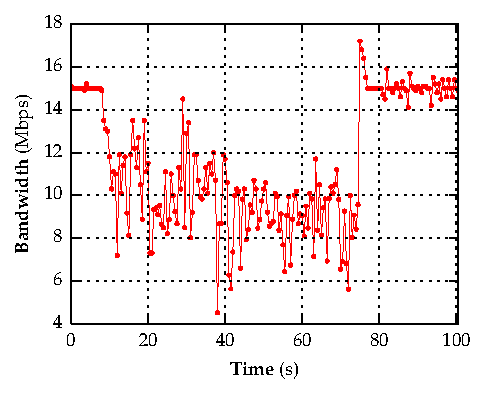
\includegraphics[width=0.75\columnwidth]{./figures/ChannelBWGraph.pdf}
  \vspace*{-0.1in}
  \caption{Bandwidth between $A$ and $D_1$ after jamming (8.5~s) and
  channel switching (75~s).}
  \label{fig:bw}
  \vspace*{-0.1in}
\end{figure}

\section{Open Challenges}
\label{sec-challenges}

\subsection{Implementing CANSAS Algorithms}

PocketSniffer allows the proposed CANSAS spectrum assignment algorithms
described in the next sections to be implemented at multiple places within
the WLAN by having agents subscribing to measurement streams generated by
PocketSniffer clients. For a small home WLAN, a programmable AP may subscribe
to the results of asynchronous queries as well as issue synchronous queries.
For a large infrastructure WLAN, programmable APs may perform local
adaptation by issuing synchronous queries while a central controller
configures all APs using measurements from asynchronous queries.

\XXXnote{GWA: Write more here...}

\subsection{Incentivizing Installation}

To avoid interfering with active terminals, CANSAS utilizes idle smartphones
to perform measurements about the channel conditions experienced by nearby
active terminals as well as performing exploration of other available
spectrum. To incentivize these measurements, SPs using PocketSniffer may
require or suggest that users install the PocketSniffer app. Requiring
terminals to submit measurements may be appropriate for SPs operating
corporate or campus WLANs where terminals are likely to repeatedly utilize
the network over an extended period of time, and where the authentication
typically required by the SP to access the network can naturally identify
relationships between terminals. These SPs may require installing the
PocketSniffer app as part of a network registration process and deny service
to terminals used by clients that fail to install the app or fail to continue
providing measurements. For each client operating a set of
terminals---attaching a smartphone, laptop, and tablet to the PocketSniffer
WLAN---a single instance of the PocketSniffer app running on their single
smartphone is sufficient to provide measurements allowing all of their other
terminals to access the WLAN.

For temporary sessions at wireless ``hotspots'', it may be more appropriate
for the SP to suggest---but not require---installing the PocketSniffer app
and provide improved quality-of-service to clients who do so, effectively
incentivizing clients by trading measurements for bandwidth. However, SPs
that operate multiple WLANs serving mobile clients, such as Boingo, may want
to require measurements from long-term subscriber or integrate PocketSniffer
into their preexisting apps such as the Boingo Wifi
Finder~\cite{boingo-playstore-url}.

\subsection{Validating Measurements}
\label{subsec-validation}

The CANSAS adaptation algorithms described next require accurate measurements
to achieve their goals. When apps compete for available spectrum, they may
have an incentive to try to manipulate the network using false measurements,
or may want to avoid the energy drain of performing measurements. When
multiple WLANs attempt to cooperate, they may have an incentive to provide
false data to each other. From the perspective of designing a network to
resist these behaviors we do not distinguish between malicious and lazy
terminals. Instead, we focus on designing PocketSniffer allowing validation
of terminal measurements that will identify both types of bad behavior. We
briefly describe several of these approaches below.

\subsubsection{Exploiting network control:\space} The easiest way for the
WLAN to detect incorrect measurements is by manipulating the
measurements using trusted devices such as APs controlled as part of
the WLAN. As an example, to prevent terminals from returning fake scan
information, PocketSniffer APs include a random nonce in each beacon
message which terminals must report as part of their scan results,
allowing the SP to verify that the terminal actually heard the scan it
is claiming to have measured. The WLAN may also manipulate the power
levels of APs to verify that these changes are reflected by terminal
measurements, to prevent the case where a terminal will incorrectly
report a low signal strength from an AP to try and force it to
increase its transmission power. Similar techniques can be applied to
verify detailed measurements, since the messages terminals overhear
can be validated by a APs controlled by the SP.

\subsubsection{Comparing terminal measurements:\space} A second approach
assuming that most terminals will cooperate with PocketSniffer is to compare
measurements from several different terminals. Without a large number of
co-located terminals to compare against it may be difficult to immediately
identify false measurements, but over time noncooperative terminals may be
identified through reputation mechanisms.

\subsubsection{Utilizing mutual observability:\space} Finally, when
considering cooperation between multiple SPs operating their own independent
WLANs we will explore the concept of \textit{mutual observability} as the
basis for establishing trust between self-interested SPs. Mutual
observability refers to the fact that although the SPs are operating
independent networks, there must be areas where their coverage overlap---if
not, there would be no need for them to coordinate spectrum allocations. This
means that there are events that should be visible to APs in both WLANs,
potentially providing a source of mutually-verifiable information to the SPs
as they attempt to cooperate.

\subsection{Controlling Client Energy Consumption}
\label{subsec-energy}

We are exploring several ways to address the energy overhead of performing
detailed spectrum utilization measurements. One is to limit these
measurements to support synchronous adaptation by active terminals operated
by the same client: i.e., by Bob's smartphone only to help Bob's laptop
locate a better channel in the example above. In the second part of the
example, if Bob has forgotten his smartphone, Alice's device may be unwilling
to incur the battery drain necessary to help Bob and only agree to provide
scan results rather than detailed channel utilization measurements. A second
approach is to ensure that the algorithms triggering synchronous data
collection only request detailed measurements when needed. Finally, the
PocketSniffer app includes an energy cap applied over each charging session
limiting the total energy clients will devote to PocketSniffer measurements.
Once this limit is exhausted, the client will not contribute measurements in
response to synchronous queries or perform detailed measurements.


\section{Related Work}
\label{sec:related}

Using client side measurements to either monitor or reconfigure
wireless networks has received a lot of attention in the recent
years. Mishra \textit{et al.}  proposed to collect client-side
measurements called \textit{site-reports}, which represent the client's
visibility to near-by APs and other devices. This information is then used to determine AP channel
assignment~\cite{mishra:mccr2005,dasilva:mswim2008,mishra:mobicom2006},
or joint channel assignment and terminal
association~\cite{mishra:infocom2006}. Sen \textit{et al.} proposed to
use mobile devices to measure and improve the performance of wide-area
cellular networks~\cite{sen2011can}. Finally, the DARPA
RadioMap~\cite{radiomap} project aims to provide real-time awareness of
radio spectrum using idle radios on user devices.

Our proposed approach differs from existing ones in the following
aspects. First, we identify smartphones as an ideal vantage point for
both long-term network monitoring and short-term network
reconfiguration, due to their \textit{always on } and \textit{mostly
  idle} nature. Second, we distinguish between active and passive
clients and propose to only collect measurements from passive clients,
and exploit device proximity detection to jointly optimize network
performance for both. Third, we consider incentives for clients to
provide measurement data and measurement validation mechanisms, which
are missing in previous works.

\section{Conclusions}
\label{sec-conclusions}

Today millions of smartphones represent a pervasive, highly-available, but
also woefully-underutilized wireless monitoring network. We have presented
the \PS{} system which harnesses the power of always-on but mostly-idle
smartphones to improve network performance for nearby active clients by using
network measurements to drive both short-term network adaptation and
long-term monitoring and debugging.

%\section{Achknowlegement}
\label{sec:ack}



\clearpage
\balance
{%
\bibliographystyle{acm}
\bibliography{references}
}
\end{document}
